\documentclass[aspectratio=169,10pt]{beamer}

% --- PACKAGES DE BASE ---
\usepackage[utf8]{inputenc}
\usepackage[T1]{fontenc}
\usepackage{lmodern}
\usepackage[french]{babel}
\usepackage{amsmath,amssymb,amsfonts}
\usepackage{graphicx}
\usepackage{booktabs}
\usepackage{tabularx}
\usepackage{multirow}

% --- CHARTE GRAPHIQUE INSEA ---
\definecolor{inseaBlue}{RGB}{20, 55, 90}
\definecolor{inseaGold}{RGB}{185, 140, 40}
\definecolor{inseaDark}{RGB}{15, 30, 50}
\definecolor{inseaLight}{RGB}{240, 245, 250}
\definecolor{cardBg}{RGB}{248, 250, 252}

\usetheme{Madrid}
\usecolortheme{whale}

\setbeamercolor{palette primary}{bg=inseaBlue,fg=white}
\setbeamercolor{palette secondary}{bg=inseaBlue!85,fg=white}
\setbeamercolor{palette tertiary}{bg=inseaDark,fg=white}
\setbeamercolor{structure}{fg=inseaBlue}
\setbeamercolor{title}{bg=inseaBlue,fg=white}
\setbeamercolor{frametitle}{bg=inseaBlue,fg=white}
\setbeamercolor{block title}{bg=inseaBlue,fg=white}
\setbeamercolor{block body}{bg=cardBg,fg=black}
\setbeamercolor{block title example}{bg=inseaGold!90!black,fg=white}
\setbeamercolor{block body example}{bg=inseaGold!10,fg=black}
\setbeamercolor{block title alert}{bg=red!80!black,fg=white}
\setbeamercolor{block body alert}{bg=red!5,fg=black}

\setbeamertemplate{navigation symbols}{}
\setbeamertemplate{footline}{
    \leavevmode%
    \hbox{%
    \begin{beamercolorbox}[wd=.333333\paperwidth,ht=2.25ex,dp=1ex,left,leftskip=2ex]{palette tertiary}%
        \textbf{INSEA} | Machine Learning S5
    \end{beamercolorbox}%
    \begin{beamercolorbox}[wd=.333333\paperwidth,ht=2.25ex,dp=1ex,center]{palette secondary}%
        Mini-Projet 02 : UCI Dry Bean
    \end{beamercolorbox}%
    \begin{beamercolorbox}[wd=.333333\paperwidth,ht=2.25ex,dp=1ex,right,rightskip=2ex]{palette primary}%
        \insertframenumber{} / \inserttotalframenumber
    \end{beamercolorbox}}%
    \vskip0pt%
}

\addtobeamertemplate{block begin}{\vspace{-0.3ex}}{\vspace{-0.2ex}}
\addtobeamertemplate{block example begin}{\vspace{-0.3ex}}{\vspace{-0.2ex}}
\addtobeamertemplate{block alert begin}{\vspace{-0.3ex}}{\vspace{-0.2ex}}

% --- METADONNEES ---
\title[\textbf{Classification UCI Dry Bean}]{\textbf{Reconnaissance Automatisée de Variétés de Haricots Secs par Apprentissage Supervisé}}
\subtitle{Étude Comparative de Cinq Architectures sur le Dataset UCI Dry Bean}
\author[\textbf{Équipe ML (DSE)}]{\textbf{Équipe Projet Machine Learning (DSE)} \\ \small Youssef FATIMI \quad Hamza BALLA \quad Mohamed Yahya SAFADI \quad Ayoub ELHANAFI}
\institute[\textbf{INSEA}]{\textbf{Institut National de Statistique et d\'Économie Appliquée (INSEA)}}
\date{Année Universitaire 2026--2027}

\begin{document}

% ==============================================================================
% SLIDE 1 : TITRE
% ==============================================================================
\begin{frame}[plain]
    \centering
    \vspace{-0.2cm}
    \begin{beamercolorbox}[sep=8pt,center,rounded=true,shadow=true]{title}
        {\usebeamerfont{title}\Large\textbf{Reconnaissance Automatisée de Variétés de Haricots Secs\\ par Apprentissage Supervisé}}\par
        \vskip0.3em
        {\usebeamerfont{subtitle}\normalsize\textit{Étude Comparative de Cinq Architectures sur le Dataset UCI Dry Bean}\par}
    \end{beamercolorbox}
    
    \vskip0.35cm
    {\small\textbf{Équipe Projet Machine Learning (DSE) :}}\par
    \vskip0.12cm
    {\footnotesize Youssef \textbf{FATIMI} \quad Hamza \textbf{BALLA} \quad Mohamed Yahya \textbf{SAFADI} \quad Ayoub \textbf{ELHANAFI}}\par
    \vskip0.18cm
    {\footnotesize \textit{Sous la direction académique de :} \textbf{Pr. Saidi}}\par
    \vfill
    {\footnotesize Année Universitaire 2026--2027}\par
    \vskip0.12cm
    \IfFileExists{figures/logo.png}{%
        \includegraphics[height=1.0cm,keepaspectratio]{figures/logo.png}\par\vskip0.1cm%
    }{%
        \vspace{1.0cm}%
    }
    
    {\small\textbf{\color{inseaBlue}Institut National de Statistique et d'Économie Appliquée (INSEA)}}\par
    \vspace{0.15cm}
    \note{
        \textbf{[00:00 - 00:45] Introduction :}
        Bonjour Monsieur le Professeur, chers collègues. Nous vous présentons aujourd'hui les conclusions de notre mini-projet de Machine Learning consacré à la reconnaissance automatisée de sept variétés de haricots secs sur le corpus de référence UCI Dry Bean.
        Notre démarche collective a répondu strictement aux exigences du cahier des charges : concevoir un protocole expérimental étanche avec zéro fuite d'information, valider empiriquement le rôle de la standardisation par une expérience d'ablation, et benchmarker de façon équitable cinq architectures supervisées.
    }
\end{frame}

% ==============================================================================
% SLIDE 2 : CONTEXTE ET PROBLEMATIQUE
% ==============================================================================
\begin{frame}{1. Contexte Métier \& Problématique Scientifique}
    \begin{columns}[T]
        \begin{column}{0.52\textwidth}
            \begin{block}{\textbf{Contexte Métier \& Défi Industriel}}
                \small
                \begin{itemize}
                    \item Le contrôle de pureté variétale des légumineuses est un enjeu agronomique et commercial majeur.
                    \item Le tri manuel traditionnel est subjectif, lent et coûteux.
                    \item \textbf{Objectif :} Automatiser la reconnaissance des 7 variétés par apprentissage supervisé \textbf{sans traiter directement les images}.
                \end{itemize}
            \end{block}
            \vspace{0.15cm}
            \begin{alertblock}{\textbf{Questions Centrales du Cahier des Charges}}
                \small
                \begin{enumerate}
                    \item \textbf{Quels modèles} distinguent le mieux les sept variétés ?
                    \item \textbf{Quelles classes} restent les plus difficiles à reconnaître ?
                \end{enumerate}
            \end{alertblock}
        \end{column}
        \begin{column}{0.46\textwidth}
            \begin{block}{\textbf{Périmètre des Cinq Modèles Étudiés}}
                \centering
                \small
                \begin{itemize}
                    \item \textbf{Régression Logistique Multiclasse} (Softmax $L_2$)
                    \item \textbf{K-Plus Proches Voisins} (KNN Géométrique)
                    \item \textbf{Arbre de Décision} (CART)
                    \item \textbf{Forêt Aléatoire} (Random Forest par bagging)
                    \item \textbf{Support Vector Machines} (SVM Linéaire \& RBF)
                \end{itemize}
            \end{block}
            \vspace{0.15cm}
            \begin{exampleblock}{\textbf{Approche TDD \& Rigueur Scientifique}}
                \footnotesize Validation empirique systématique : chaque hypothèse théorique est confirmée par des mesures quantifiées sur le jeu de test scellé.
            \end{exampleblock}
        \end{column}
    \end{columns}
    \note{
        \textbf{[00:45 - 01:30] Problématique :}
        Le tri manuel des semences de haricots altère la valeur marchande des récoltes.
        Le sujet nous pose deux questions fondamentales : identifier l'algorithme le plus performant parmi cinq grandes familles du cours, et déterminer les classes intrinsèquement confondues.
        Nous avons développé ces cinq architectures dans un cadre méthodologique étanche et reproductible.
    }
\end{frame}

% ==============================================================================
% SLIDE 3 : JEU DE DONNEES ET REPARTITION DES CLASSES
% ==============================================================================
\begin{frame}{2. Description du Corpus UCI Dry Bean \& Déséquilibre}
    \begin{columns}[T]
        \begin{column}{0.52\textwidth}
            \begin{block}{\textbf{Corpus UCI Dry Bean \& Métrique Reine}}
                \scriptsize
                $N = \mathbf{13\,611}$ grains $\cdot$ 16 descripteurs $\cdot$ Asymétrie de 1 à 6.8.\\
                Le \textbf{F1-score Macro} $F_{1,\text{macro}} = \frac{1}{K}\sum F_{1,k}$ est le critère cardinal.
            \end{block}
            \vspace{0.15cm}
            \begin{block}{\textbf{Répartition des 7 Variétés dans le Corpus}}
                \centering
                \scriptsize
                \begin{tabular}{@{}llcc@{}}
                    \toprule
                    \textbf{Variété} & \textbf{Code} & \textbf{Effectif} & \textbf{Proportion} \\
                    \midrule
                    Dermason & \texttt{DERMASON} & 3\,546 & 26.05\,\% \\
                    Sira     & \texttt{SIRA}     & 2\,636 & 19.37\,\% \\
                    Seker    & \texttt{SEKER}    & 2\,027 & 14.89\,\% \\
                    Horoz    & \texttt{HOROZ}    & 1\,928 & 14.16\,\% \\
                    Cali     & \texttt{CALI}     & 1\,630 & 11.98\,\% \\
                    Barbunya & \texttt{BARBUNYA} & 1\,322 & 9.71\,\%  \\
                    Bombay   & \texttt{BOMBAY}   & 522   & 3.84\,\%  \\
                    \midrule
                    \textbf{Total} & \textbf{7 classes} & \textbf{13\,611} & \textbf{100.00\,\%} \\
                    \bottomrule
                \end{tabular}
            \end{block}
        \end{column}
        \begin{column}{0.46\textwidth}
            \centering
            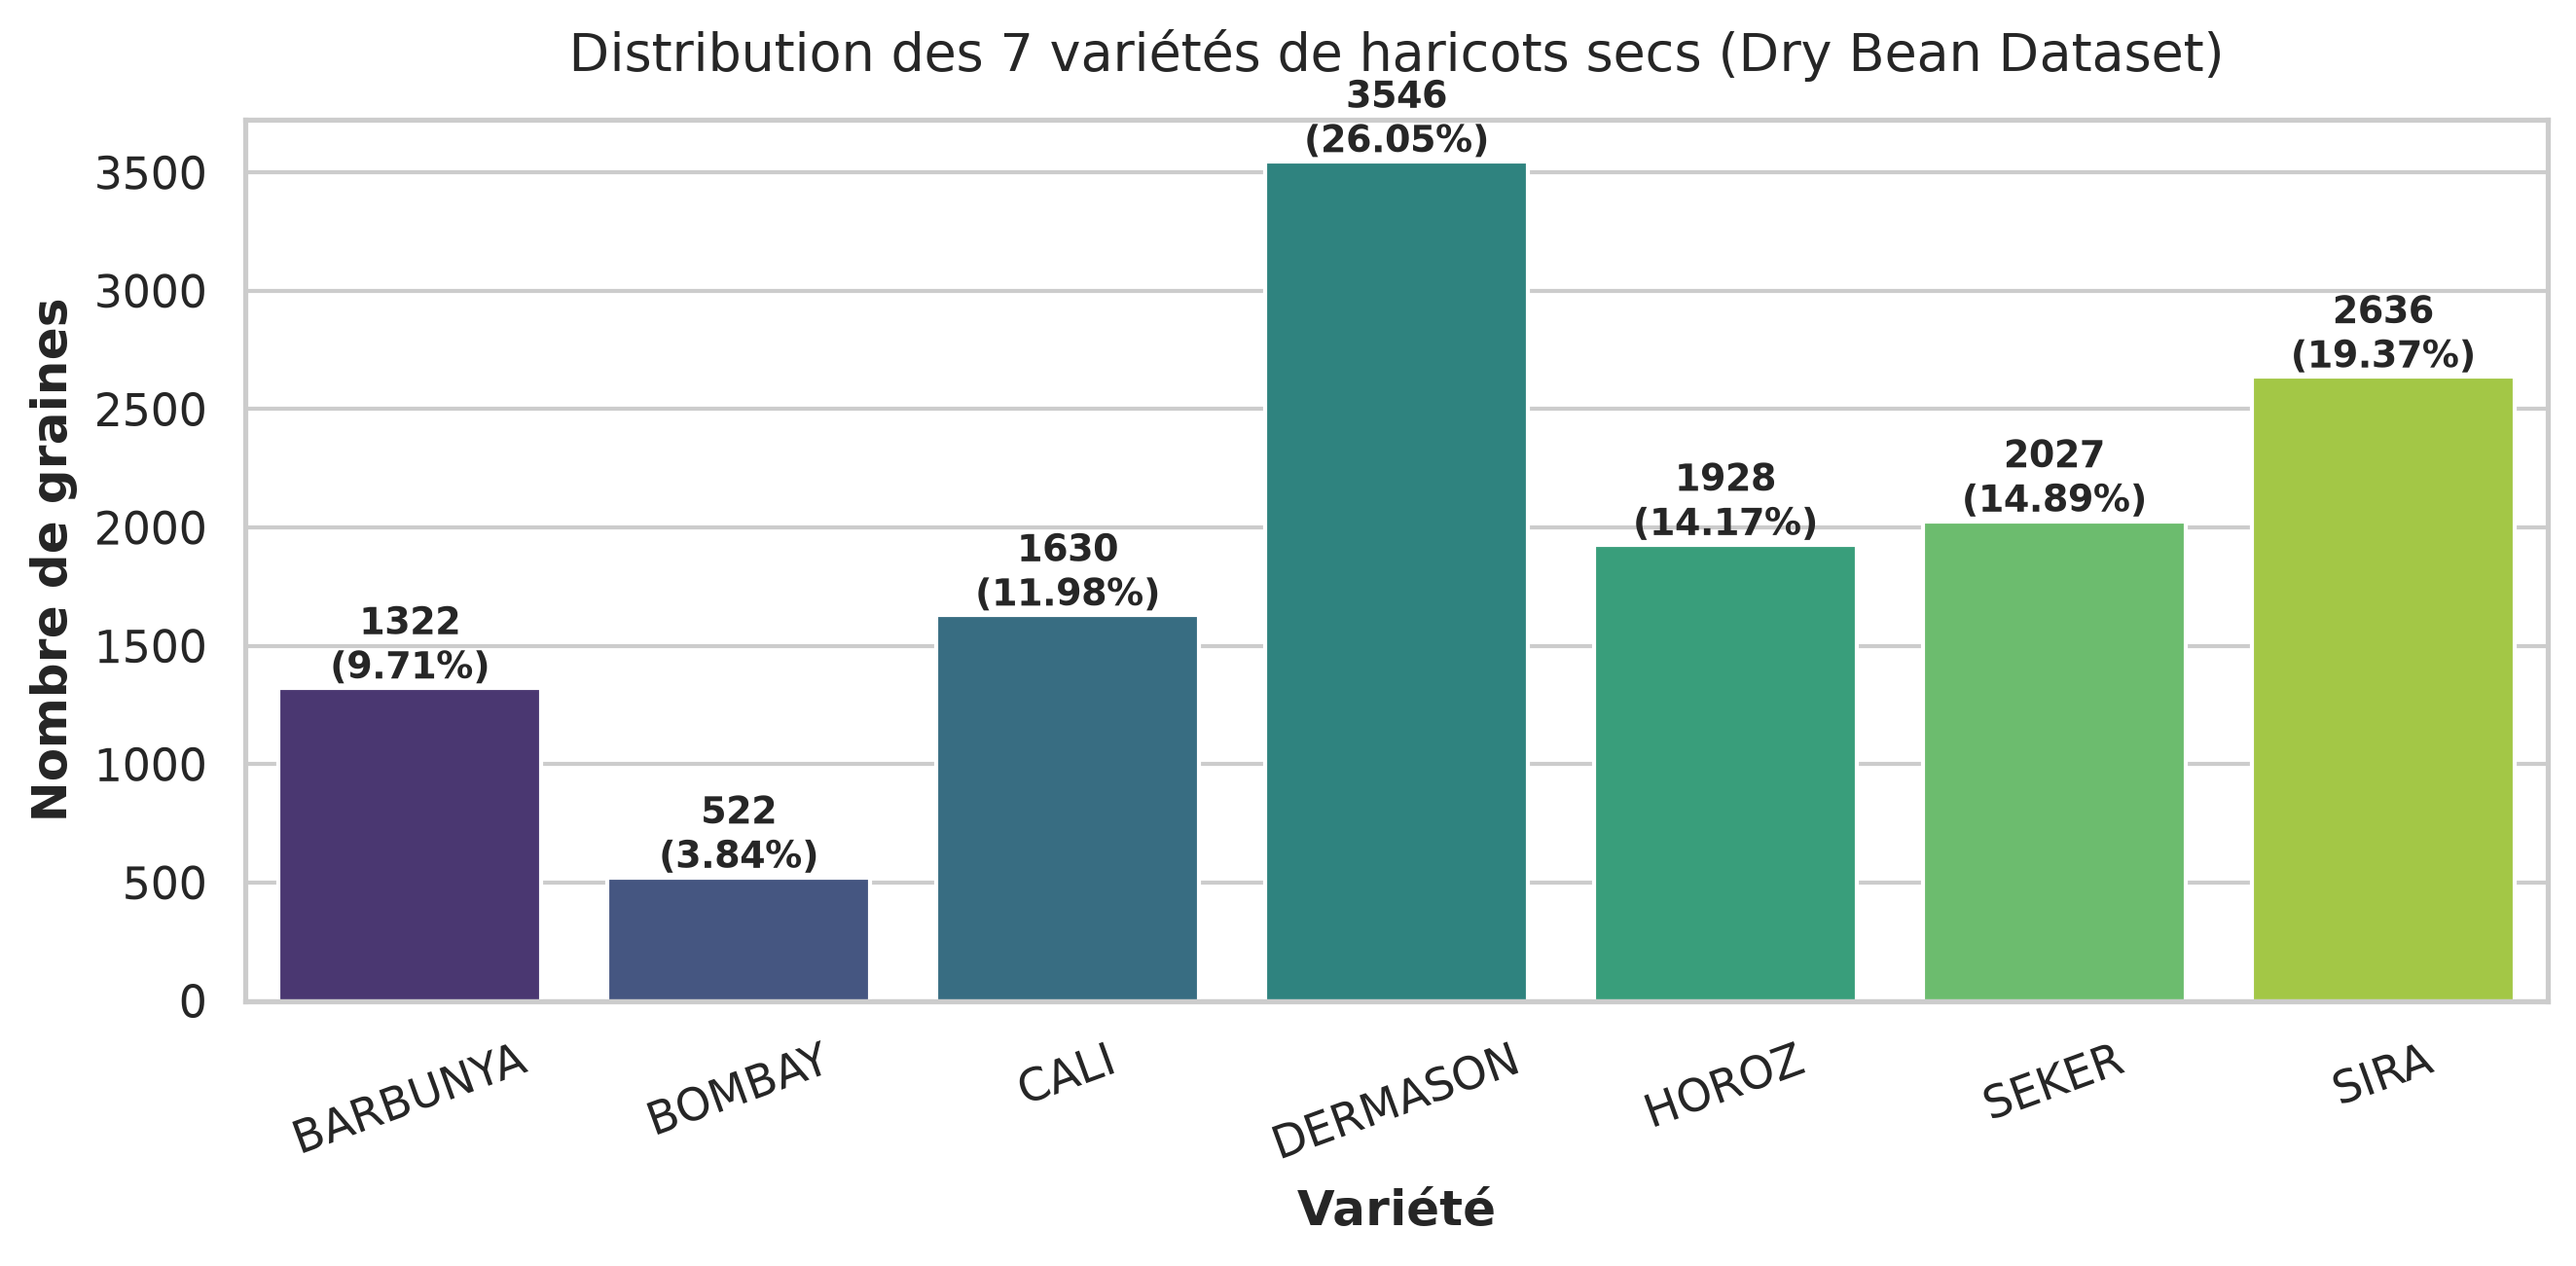
\includegraphics[width=\textwidth,height=4.6cm,keepaspectratio]{figures/01_eda_classes_distribution.png}\\[0.1cm]
            {\scriptsize\textcolor{inseaBlue}{\textbf{Figure 1 :}} \textit{Distribution des effectifs par variété de haricot}}
        \end{column}
    \end{columns}
    \note{
        \textbf{[01:30 - 02:30] Données \& Déséquilibre :}
        Le dataset comporte 13 611 grains et 16 descripteurs sans valeurs manquantes.
        Comme l'illustre la Figure 1 et le tableau de répartition, nous avons une asymétrie marquée : Dermason représente 26% alors que Bombay n'en représente que 3.8%.
        L'Accuracy brute serait trompeuse. Conformément aux consignes, nous privilégions le F1-score Macro qui accorde le même poids à chaque variété.
    }
\end{frame}

% ==============================================================================
% SLIDE 4 : DISTRIBUTIONS MORPHOLOGIQUES ET INVARIANTS
% ==============================================================================
\begin{frame}{3. Distributions Morphologiques \& Invariants Physiques}
    \begin{columns}[T]
        \begin{column}{0.48\textwidth}
            \begin{block}{\textbf{Les 4 Invariants Physiques Fondamentaux}}
                \footnotesize
                \begin{enumerate}
                    \item \textbf{Bombay (Géant) :} Aire médiane $\approx 173\,000$ px² (vs $< 70\,000$ px² pour les autres). Séparabilité quasi linéaire immédiate.
                    \item \textbf{Horoz (Allongé) :} Ratio d'aspect ($> 2.1$) et excentricité maximaux : silhouette cylindrique nette.
                    \item \textbf{Seker (Sphérique) :} Compacité et circularité maximales ($\approx 0.94$).
                    \item \textbf{Dermason / Sira (Piège) :} Tailles et formes presque confondues : \textbf{foyer d'erreur majeur attendu}.
                \end{enumerate}
            \end{block}
            \vspace{0.15cm}
            \begin{exampleblock}{\textbf{Multicolinéarité Dimensionnelle}}
                \footnotesize Corrélations $r \ge 0.98$ entre \texttt{Area}, \texttt{Perimeter} et \texttt{ConvexArea} $\rightarrow$ impose une régularisation de crête ($L_2$).
            \end{exampleblock}
        \end{column}
        \begin{column}{0.50\textwidth}
            \centering
            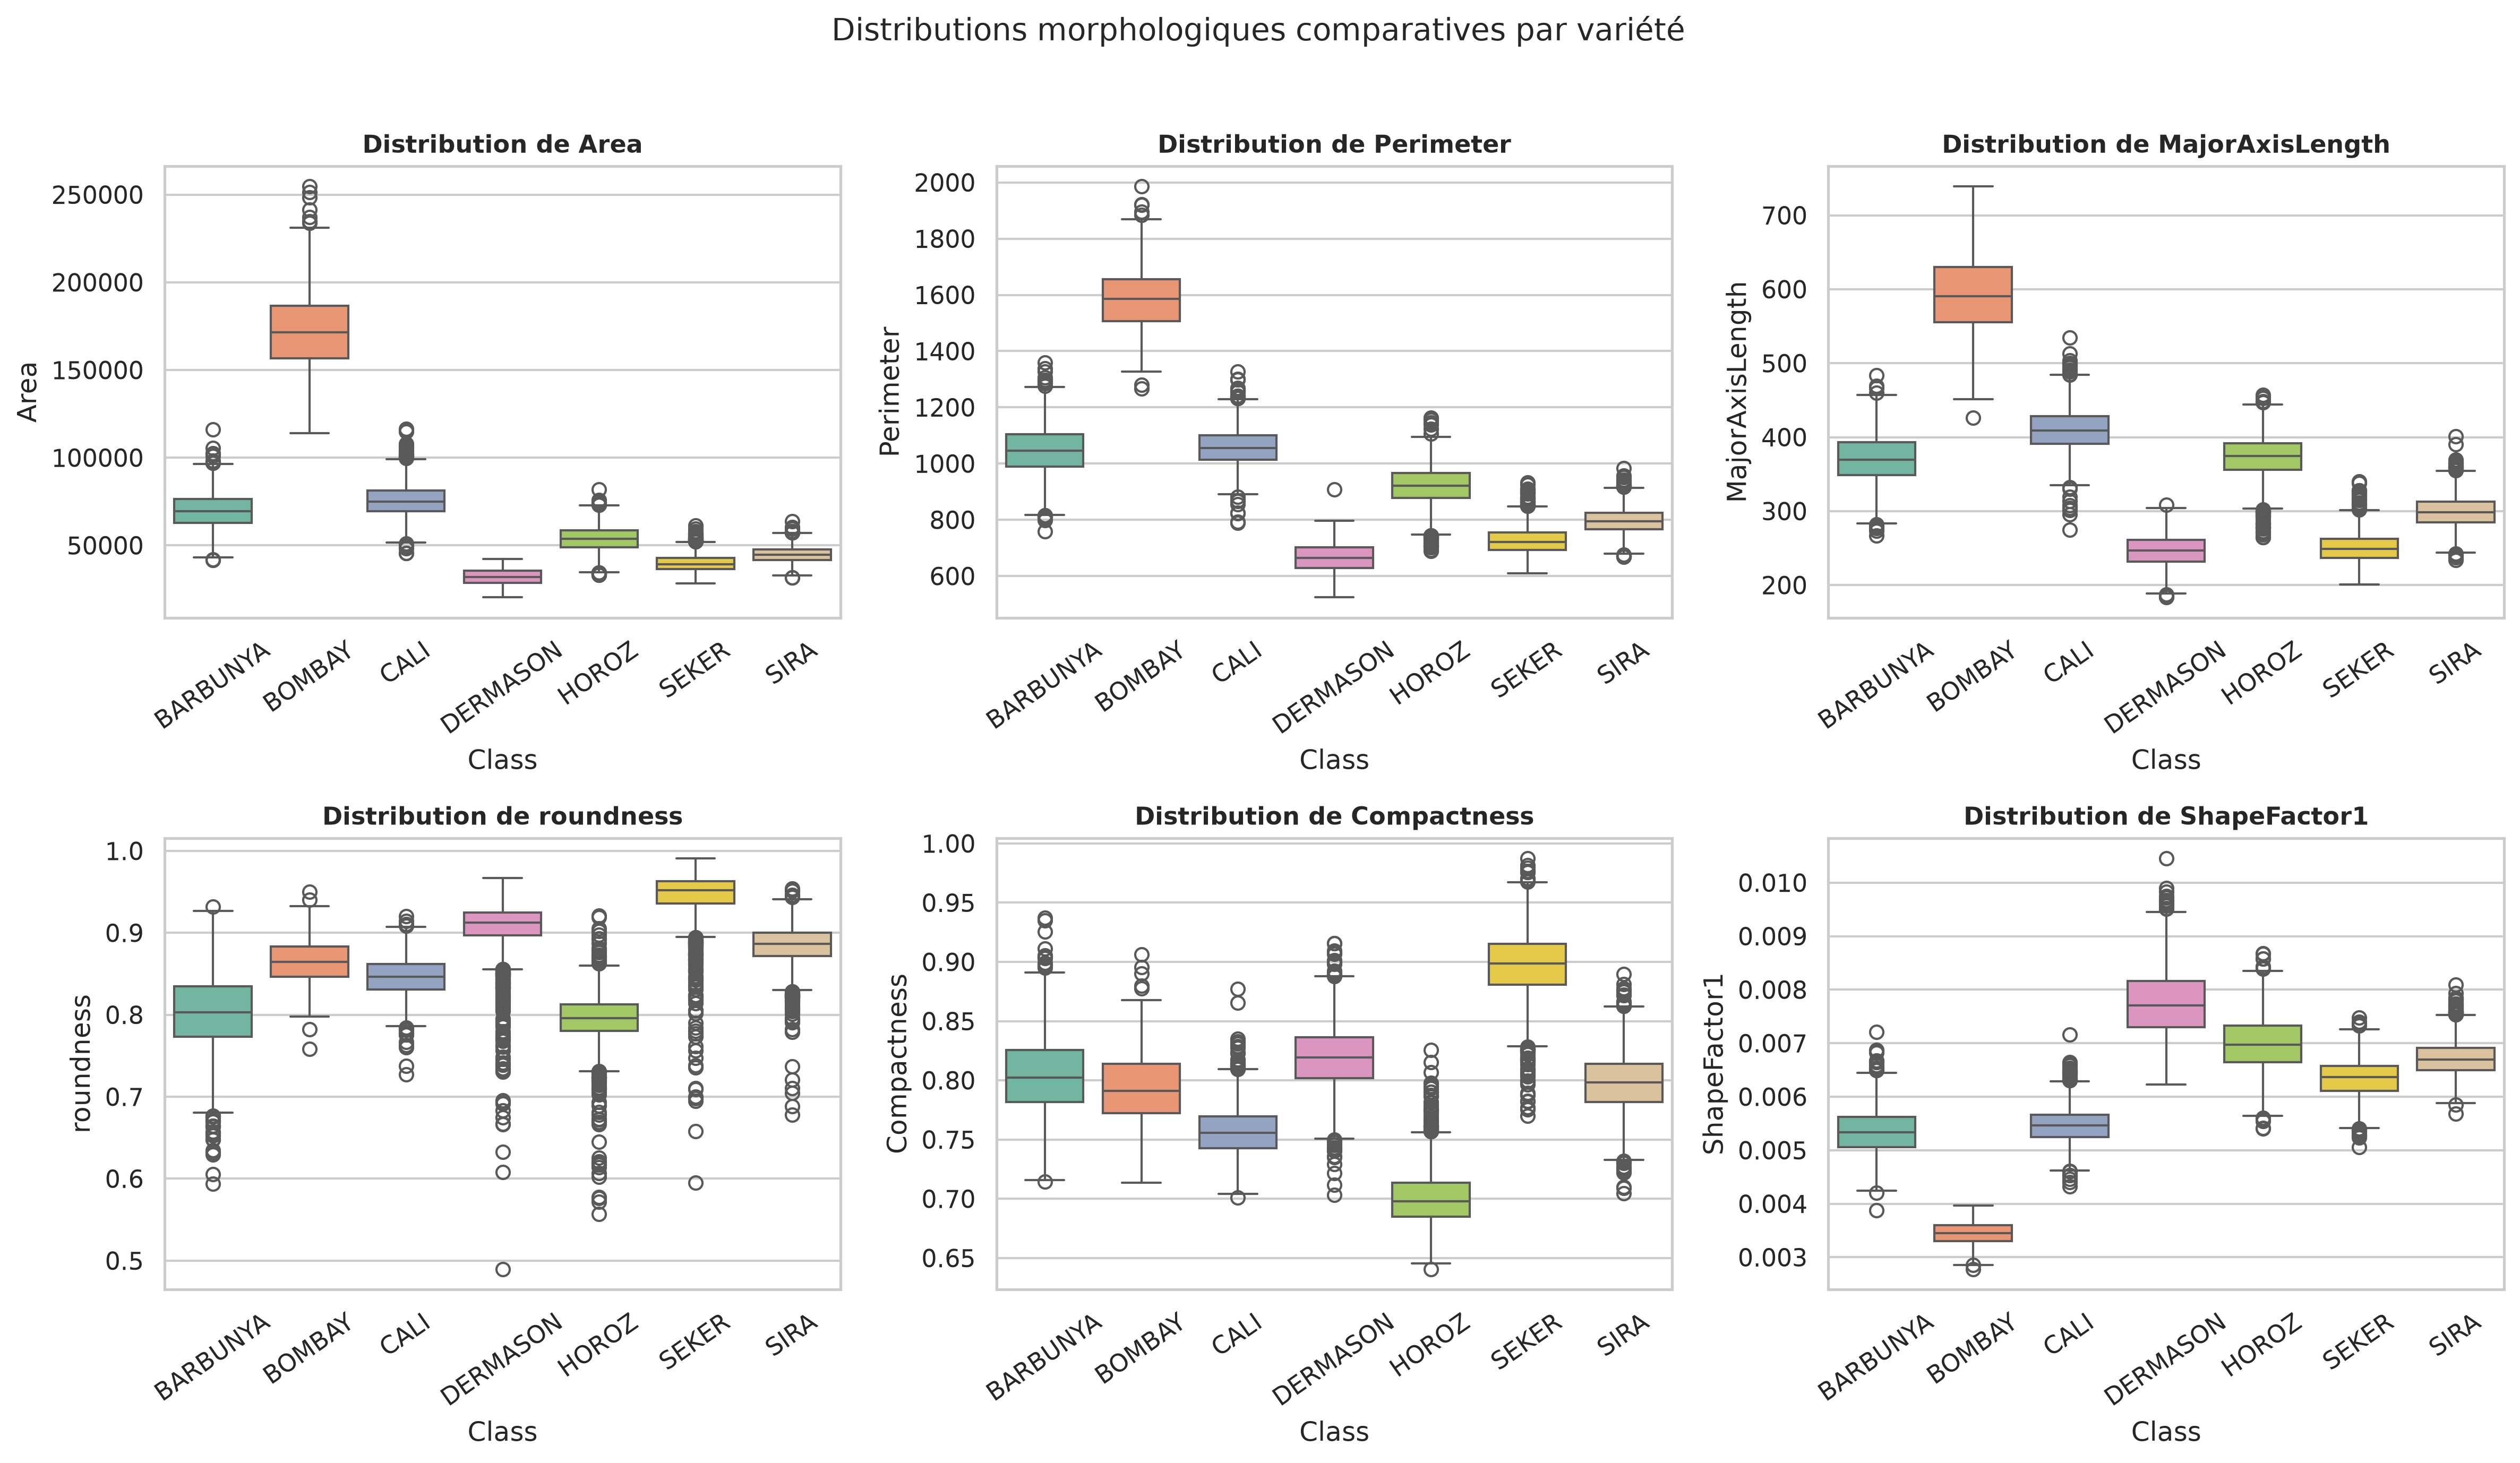
\includegraphics[width=\textwidth,height=4.2cm,keepaspectratio]{figures/02_eda_morphological_boxplots.png}\\[0.1cm]
            {\scriptsize\textcolor{inseaBlue}{\textbf{Figure 2 :}} \textit{Distributions comparatives des descripteurs morphologiques}}
        \end{column}
    \end{columns}
    \note{
        \textbf{[02:30 - 03:30] Distributions Morphologiques :}
        La Figure 2 met en évidence la signature géométrique de chaque variété.
        Bombay se détache totalement par sa taille colossale.
        Horoz s'isole par son élongation et Seker par sa compacité sphérique.
        En revanche, notez bien Dermason et Sira sur les boxplots : leurs distributions se chevauchent de manière critique, préfigurant la frontière Bayesienne la plus complexe du problème.
    }
\end{frame}

% ==============================================================================
% SLIDE 5 : PROTOCOLE EXPERIMENTAL ET ZERO DATA LEAKAGE
% ==============================================================================
\begin{frame}{4. Protocole Expérimental Partagé (Règle d'Or)}
    \begin{columns}[T]
        \begin{column}{0.52\textwidth}
            \begin{block}{\textbf{La Règle d'Or du Protocole Partagé}}
                \small
                \begin{itemize}
                    \item \textbf{Graine Aléatoire Universelle :} $\texttt{SEED} = 42$ commune.
                    \item \textbf{Partitionnement Étanche :} 80\,\% Train ($N=10\,888$) / 20\,\% Test ($N=2\,723$), avec stratification stricte.
                    \item \textbf{Validation Croisée 5-Plis :} \texttt{StratifiedKFold} sur le train pour tous les \texttt{GridSearchCV}.
                    \item \textbf{Isolation du Test Set :} Évalué une seule et unique fois à la fin.
                \end{itemize}
            \end{block}
            \vspace{0.15cm}
            \begin{alertblock}{\textbf{Garantie Zéro Fuite (\textit{Zero Data Leakage})}}
                \footnotesize Le \texttt{StandardScaler} est systématiquement encapsulé dans un \texttt{Pipeline} Scikit-Learn : appris (\texttt{fit}) \textbf{exclusivement sur les plis d'entraînement internes}.
            \end{alertblock}
        \end{column}
        \begin{column}{0.46\textwidth}
            \begin{block}{\textbf{Vérification de la Stratification Train / Test}}
                \centering
                \scriptsize
                \begin{tabular}{@{}lccc@{}}
                    \toprule
                    \textbf{Variété} & \textbf{Corpus (\%)} & \textbf{Train (\%)} & \textbf{Test (\%)} \\
                    \midrule
                    Dermason & 26.05\,\% & 26.05\,\% & 26.04\,\% \\
                    Sira     & 19.37\,\% & 19.37\,\% & 19.35\,\% \\
                    Seker    & 14.89\,\% & 14.89\,\% & 14.91\,\% \\
                    Horoz    & 14.16\,\% & 14.16\,\% & 14.18\,\% \\
                    Cali     & 11.98\,\% & 11.98\,\% & 11.97\,\% \\
                    Barbunya & 9.71\,\%  & 9.71\,\%  & 9.70\,\%  \\
                    Bombay   & 3.84\,\%  & 3.84\,\%  & 3.86\,\%  \\
                    \bottomrule
                \end{tabular}
            \end{block}
            \vspace{0.1cm}
            \begin{exampleblock}{\textbf{Baseline Aléatoire Naïve}}
                \footnotesize \texttt{DummyClassifier} (stratifié) plafonne à $F_1 = \mathbf{0.1472}$.
            \end{exampleblock}
        \end{column}
    \end{columns}
    \note{
        \textbf{[03:30 - 04:15] Protocole Expérimental :}
        Pour assurer une rigueur irréprochable au sein de notre équipe, nous avons verrouillé le protocole.
        La division 80/20 respecte exactement les fréquences marginales au centième de pourcent près.
        Point capital : aucun data leakage. Le centrage-réduction est systématiquement calculé au sein d'un Pipeline Scikit-Learn pour n'être appris que sur les plis d'entraînement.
    }
\end{frame}

% ==============================================================================
% SLIDE 6 : ETUDE D'ABLATION - IMPACT DU CENTRAGE-REDUCTION
% ==============================================================================
\begin{frame}{5. Expérience d'Ablation : Impact Vital du Centrage-Réduction}
    \begin{columns}[T]
        \begin{column}{0.54\textwidth}
            \begin{block}{\textbf{Résultats de l'Ablation (CV 5-plis Train)}}
                \centering
                \scriptsize
                \begin{tabular}{@{}lccc@{}}
                    \toprule
                    \textbf{Algorithme} & \textbf{Sans Scaling} & \textbf{Avec Scaling} & \textbf{Gain (pts)} \\
                    \midrule
                    \textbf{SVM (Noyau RBF)} & 0.5983 & \textbf{0.9343} & \textcolor{green!60!black}{\textbf{+33.60}} \\
                    \textbf{KNN ($k=9$)}      & 0.7138 & \textbf{0.9355} & \textcolor{green!60!black}{\textbf{+22.17}} \\
                    \textbf{Régression Log.} & 0.7544 & \textbf{0.9329} & \textcolor{green!60!black}{\textbf{+17.85}} \\
                    \textbf{Forêt Aléatoire} & 0.9321 & 0.9321 & \textbf{0.00} \\
                    \textbf{Arbre CART}      & 0.9194 & 0.9194 & \textbf{0.00} \\
                    \bottomrule
                \end{tabular}
            \end{block}
            \vspace{0.15cm}
            \begin{alertblock}{\textbf{Verdict Expérimental}}
                \footnotesize Le centrage-réduction est \textbf{obligatoire} pour SVM, KNN et Régression Logistique, mais strictement neutre pour les arbres.
            \end{alertblock}
        \end{column}
        \begin{column}{0.44\textwidth}
            \begin{block}{\textbf{Justification Mathématique}}
                \footnotesize
                \begin{itemize}
                    \item \textbf{Modèles Métriques \& Gradients :}
                    Disparité d'échelle ($Area \approx 10^5$ vs $ShapeFactor \approx 10^{-3}$) : le calcul $\|\mathbf{x}_i - \mathbf{x}_j\|^2$ est écrasé par l'aire, annihilant le noyau gaussien.
                    \item \textbf{Modèles Arborescents (Invariance) :}
                    Coupures basées sur le critère de Gini : $x_j \le s$. Toute transformation monotone $z = \frac{x-\mu}{\sigma}$ préserve l'ordre et laisse les partitions invariantes ($\Delta = 0.00$).
                \end{itemize}
            \end{block}
        \end{column}
    \end{columns}
    \note{
        \textbf{[04:15 - 05:15] Expérience d'Ablation :}
        Voici le résultat théorique majeur confirmé par l'expérience :
        Pour le SVM RBF, l'absence de centrage-réduction entraîne un effondrement spectaculaire de 33.6 points de F1 macro ! Pour KNN, la perte dépasse 22 points.
        Pourquoi ? L'aire domine complètement le calcul de distance euclidienne.
        En revanche, observez CART et Random Forest : l'écart est strictement nul à 0.00 point près, confirmant mathématiquement l'invariance d'échelle des arbres de décision.
    }
\end{frame}

% ==============================================================================
% SLIDE 7 : MODELISATION ET HYPERPARAMETRES OPTIMAUX
% ==============================================================================
\begin{frame}{6. Modélisation \& Optimisation des 5 Architectures}
    \begin{columns}[T]
        \begin{column}{0.48\textwidth}
            \begin{block}{\textbf{1. Régression Logistique (Softmax $L_2$)}}
                \scriptsize
                $P(y = k \mid \mathbf{x}) = \frac{\exp(\mathbf{w}_k^T \mathbf{x} + b_k)}{\sum_j \exp(\mathbf{w}_j^T \mathbf{x} + b_j)}$.\\
                \textbf{Optimum :} $C^* = 100$ (solveur L-BFGS). Convergence rapide et surface convexe bien conditionnée.
            \end{block}
            \vspace{0.1cm}
            \begin{block}{\textbf{2. K-Plus Proches Voisins (KNN)}}
                \scriptsize
                Agrégation locale non paramétrique.\\
                \textbf{Optimum :} $k^* = 9$, distance euclidienne, pondération $w_i = 1/d$ (lève le flou décisionnel dense).
            \end{block}
            \vspace{0.1cm}
            \begin{block}{\textbf{3. Arbre de Décision (CART)}}
                \scriptsize
                Minimisation de l'impureté de Gini $I_G(t)$.\\
                \textbf{Optimum :} $\texttt{max\_depth}^* = 9$ (évite le sur-apprentissage précoce des arbres libres).
            \end{block}
        \end{column}
        \begin{column}{0.48\textwidth}
            \begin{block}{\textbf{4. Forêt Aléatoire (Random Forest)}}
                \scriptsize
                Ensemble de $B = 200$ arbres décorrélés par \textit{bagging} et tirage aléatoire de $\sqrt{p} = 4$ variables par nœud.\\
                \textbf{Optimum :} $n^* = 200$, $\texttt{max\_depth}^* = 15$.\\
                Réduit drastiquement la variance (+1.27 pt vs CART).
            \end{block}
            \vspace{0.1cm}
            \begin{block}{\textbf{5. Support Vector Machines (SVM RBF)}}
                \scriptsize
                Hyperplan à marge maximale avec variables souples :\\
                $\min \frac{1}{2}\|\mathbf{w}\|^2 + C\sum\xi_i \quad \text{s.t.} \quad y_i(\mathbf{w}^T\phi(\mathbf{x}_i)+b) \ge 1-\xi_i$.\\
                Noyau gaussien $K(\mathbf{x}_i, \mathbf{x}_j) = \exp(-\gamma\|\mathbf{x}_i-\mathbf{x}_j\|^2)$.\\
                \textbf{Optimum :} $C^* = 5, \quad \gamma^* = 0.1$.\\
                Courbe les frontières dans l'espace de Hilbert.
            \end{block}
        \end{column}
    \end{columns}
    \note{
        \textbf{[05:15 - 06:30] Optimisation des Modèles :}
        Chaque algorithme a fait l'objet d'un GridSearchCV 5-plis optimisant le F1 macro.
        Pour KNN, la pondération par l'inverse de la distance avec k=9 surpasse le vote uniforme.
        Pour CART, borner la profondeur à 9 stabilise les frontières.
        Pour Random Forest, 200 arbres et 4 variables par split réduisent la variance.
        Pour SVM, la combinaison C=5 et gamma=0.1 exploite la flexibilité du noyau RBF.
    }
\end{frame}

% ==============================================================================
% SLIDE 8 : GRAND BENCHMARK COMPARATIF
% ==============================================================================
\begin{frame}{7. Grand Benchmark Comparatif sur le Test Set ($N_{\text{test}} = 2\,723$)}
    \begin{block}{\textbf{Synthèse Générale des Performances Comparatives}}
        \centering
        \resizebox{\linewidth}{!}{
        \begin{tabular}{@{}llcccccr@{}}
            \toprule
            \textbf{Rang / Modèle} & \textbf{Hyperparamètres Optimaux} & \textbf{F1 CV (Train)} & \textbf{Accuracy (\%)} & \textbf{Précision} & \textbf{Rappel} & \textbf{F1 Macro} & \textbf{Inférence (ms)} \\
            \midrule
            1. \textbf{SVM (Noyau RBF)} & $C=5, \gamma=0.1$ & \textbf{0.9388} & \textbf{92.47\,\%} & \textbf{0.9366} & \textbf{0.9362} & \textbf{0.9363} & 15.2 ms \\
            2. \textbf{Régression Logistique} & $C=100$ & 0.9329 & 92.10\,\% & 0.9333 & 0.9327 & 0.9329 & \textbf{2.1 ms} \\
            3. \textbf{Random Forest} & $n=200, \texttt{depth}=15$ & 0.9365 & 92.25\,\% & 0.9325 & 0.9320 & 0.9321 & 28.4 ms \\
            4. \textbf{KNN (Pondéré)} & $k=9, \text{euclidien, distance}$ & 0.9382 & 92.18\,\% & 0.9304 & 0.9298 & 0.9300 & 45.1 ms \\
            5. \textbf{Arbre CART} & $\texttt{max\_depth}=9$ & 0.9194 & 90.56\,\% & 0.9196 & 0.9193 & 0.9194 & 0.9 ms \\
            \bottomrule
        \end{tabular}
        }
    \end{block}
    \vspace{0.15cm}
    \begin{columns}[T]
        \begin{column}{0.48\textwidth}
            \begin{alertblock}{\textbf{1. Le Sacre du SVM RBF (Champion Absolu)}}
                \footnotesize Domine sur l'ensemble des indicateurs ($F_1 = \mathbf{0.9363}$, $\text{Acc} = \mathbf{92.47\,\%}$). La marge maximale et la pénalisation $\|\mathbf{w}\|^2$ assurent la meilleure généralisation.
            \end{alertblock}
        \end{column}
        \begin{column}{0.48\textwidth}
            \begin{exampleblock}{\textbf{2. L'Efficience Record de la Régression Logistique}}
                \footnotesize Talonne le champion à seulement 0.34 pt ($F_1 = 0.9329$) tout en exécutant l'inférence en \textbf{2.1 ms} (\textbf{7x plus rapide que SVM, 21x plus rapide que KNN}).
            \end{exampleblock}
        \end{column}
    \end{columns}
    \note{
        \textbf{[06:30 - 07:30] Grand Benchmark :}
        Voici le tableau récapitulatif officiel évalué sur le jeu de test scellé.
        Le SVM à noyau RBF décroche la première place sur tous les critères.
        Mais observez la Régression Logistique : elle se place à seulement 0.34 point du champion avec un temps d'inférence exceptionnel de 2.1 ms.
        En revanche, l'arbre individuel CART accuse un retard net de 1.7 point, limité par ses découpages orthogonaux.
    }
\end{frame}

% ==============================================================================
% SLIDE 9 : ANALYSE DES PERFORMANCES PAR VARIETE
% ==============================================================================
\begin{frame}{8. Analyse Désagrégée des Performances par Variété}
    \begin{columns}[T]
        \begin{column}{0.48\textwidth}
            \begin{block}{\textbf{Enseignements par Classe (Figure 3)}}
                \small
                \begin{itemize}
                    \item \textbf{Sans-faute sur Bombay :} Score parfait de $F_1 = \mathbf{1.0000}$ pour les 5 modèles (0 faux positif, 0 faux négatif).
                    \item \textbf{Stabilité sur Horoz \& Seker :} $F_1 \ge 0.94$, captés par la compacité et l'élongation.
                    \item \textbf{Cali \& Barbunya :} Bien séparés ($F_1 \approx 0.93 - 0.94$).
                    \item \textbf{Le Pivot Dermason / Sira :} $F_1 < 0.90$. C'est ici que le SVM RBF fait la différence (+0.91 pt vs LogReg).
                \end{itemize}
            \end{block}
            \vspace{0.1cm}
            \begin{exampleblock}{\textbf{Gain vs Baselines Factices}}
                \footnotesize Nos modèles opèrent à plus de \textbf{6.3 fois au-dessus du hasard pur} (\texttt{DummyClassifier} à 0.1472).
            \end{exampleblock}
        \end{column}
        \begin{column}{0.50\textwidth}
            \centering
            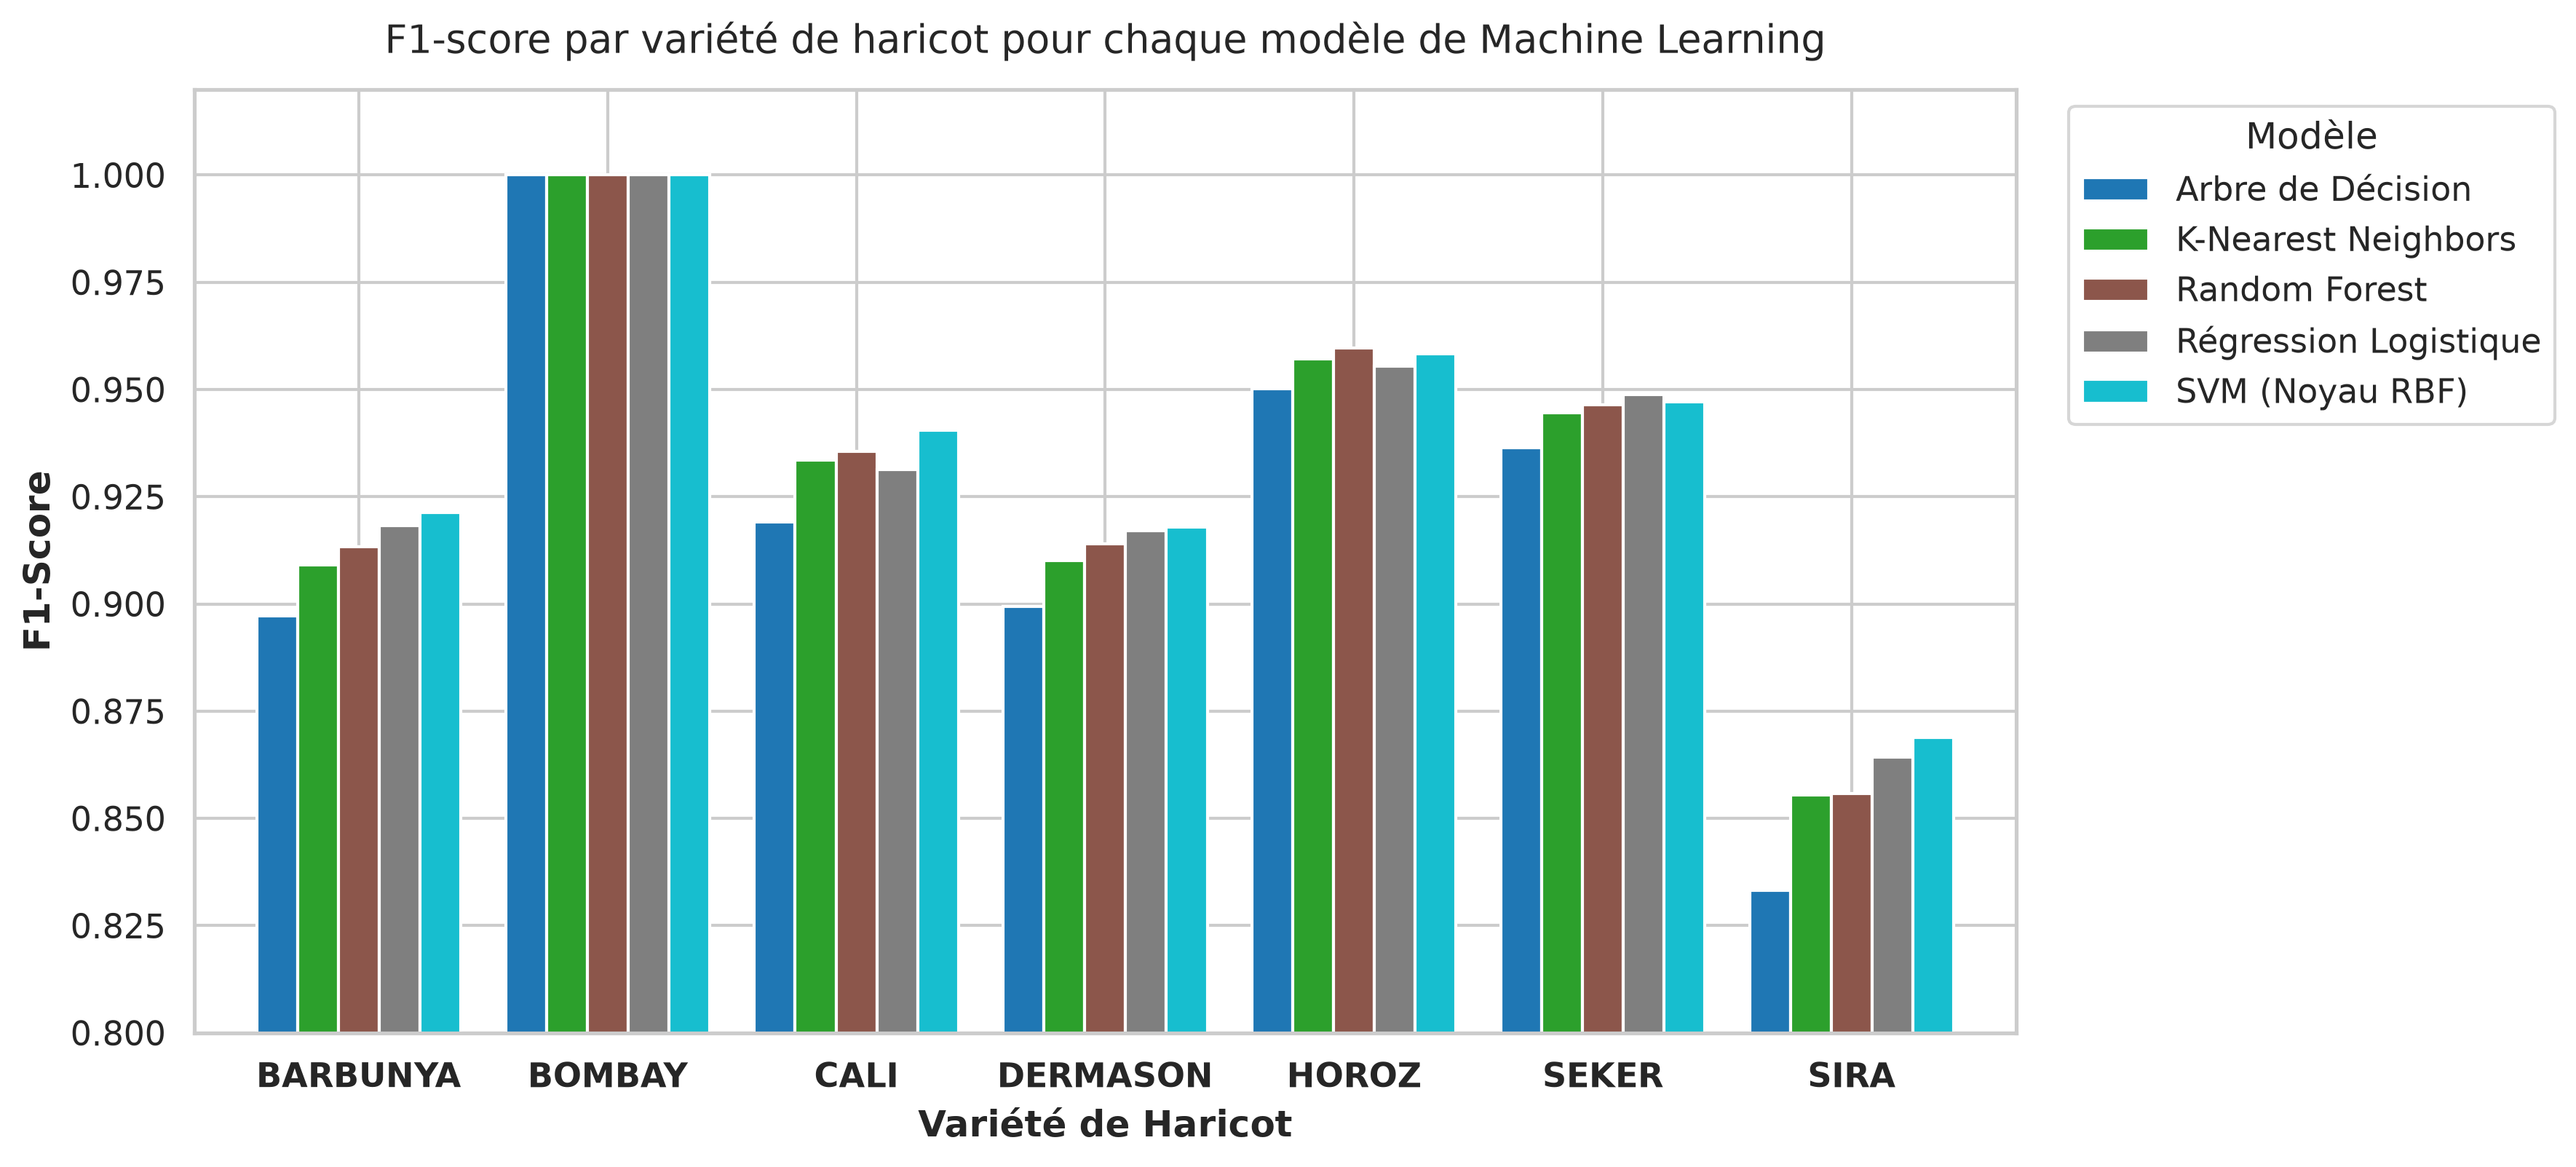
\includegraphics[width=\textwidth,height=4.6cm,keepaspectratio]{figures/06_f1_scores_per_class.png}\\[0.1cm]
            {\scriptsize\textcolor{inseaBlue}{\textbf{Figure 3 :}} \textit{Comparaison des F1-scores par classe pour les 5 modèles}}
        \end{column}
    \end{columns}
    \note{
        \textbf{[07:30 - 08:30] F1 par Variété :}
        La Figure 3 décompose les scores par variété.
        Sur Bombay, les cinq algorithmes atteignent la perfection absolue : 1.0000.
        Horoz et Seker dépassent 0.94 sans difficulté.
        La vraie bataille se joue sur Dermason et Sira : c'est sur ces deux classes que le SVM RBF creuse l'écart de près d'un point face à la régression logistique, expliquant son sacre.
    }
\end{frame}

% ==============================================================================
% SLIDE 10 : DISSECTION DES ERREURS ET LIMITE BAYESIENNE
% ==============================================================================
\begin{frame}{9. Dissection des Confusions \& Limite Bayesienne 2D}
    \begin{columns}[T]
        \begin{column}{0.48\textwidth}
            \begin{block}{\textbf{Bilan des 205 Erreurs du Champion ($7.53\,\%$)}}
                \footnotesize
                \begin{itemize}
                    \item \textbf{46.8\,\% des erreurs = Dermason $\leftrightarrow$ Sira :} 96 confusions mutuelles (52 Dermason pris pour Sira, 44 Sira pris pour Dermason).
                    \item \textbf{11.7\,\% des erreurs = Barbunya $\leftrightarrow$ Cali :} 24 grains mutuellement confondus (courbures proches).
                    \item \textbf{Zéro pollution sur Bombay :} 0 confusion.
                \end{itemize}
            \end{block}
            \vspace{0.1cm}
            \begin{alertblock}{\textbf{Limite Bayesienne Intrinsèque 2D}}
                \footnotesize Dans l'espace morphologique 2D, les distributions de Dermason et Sira \textbf{se chevauchent physiquement}. Aucun séparateur géométrique ne peut lever cette ambiguïté sans variable de couleur.
            \end{alertblock}
        \end{column}
        \begin{column}{0.50\textwidth}
            \centering
            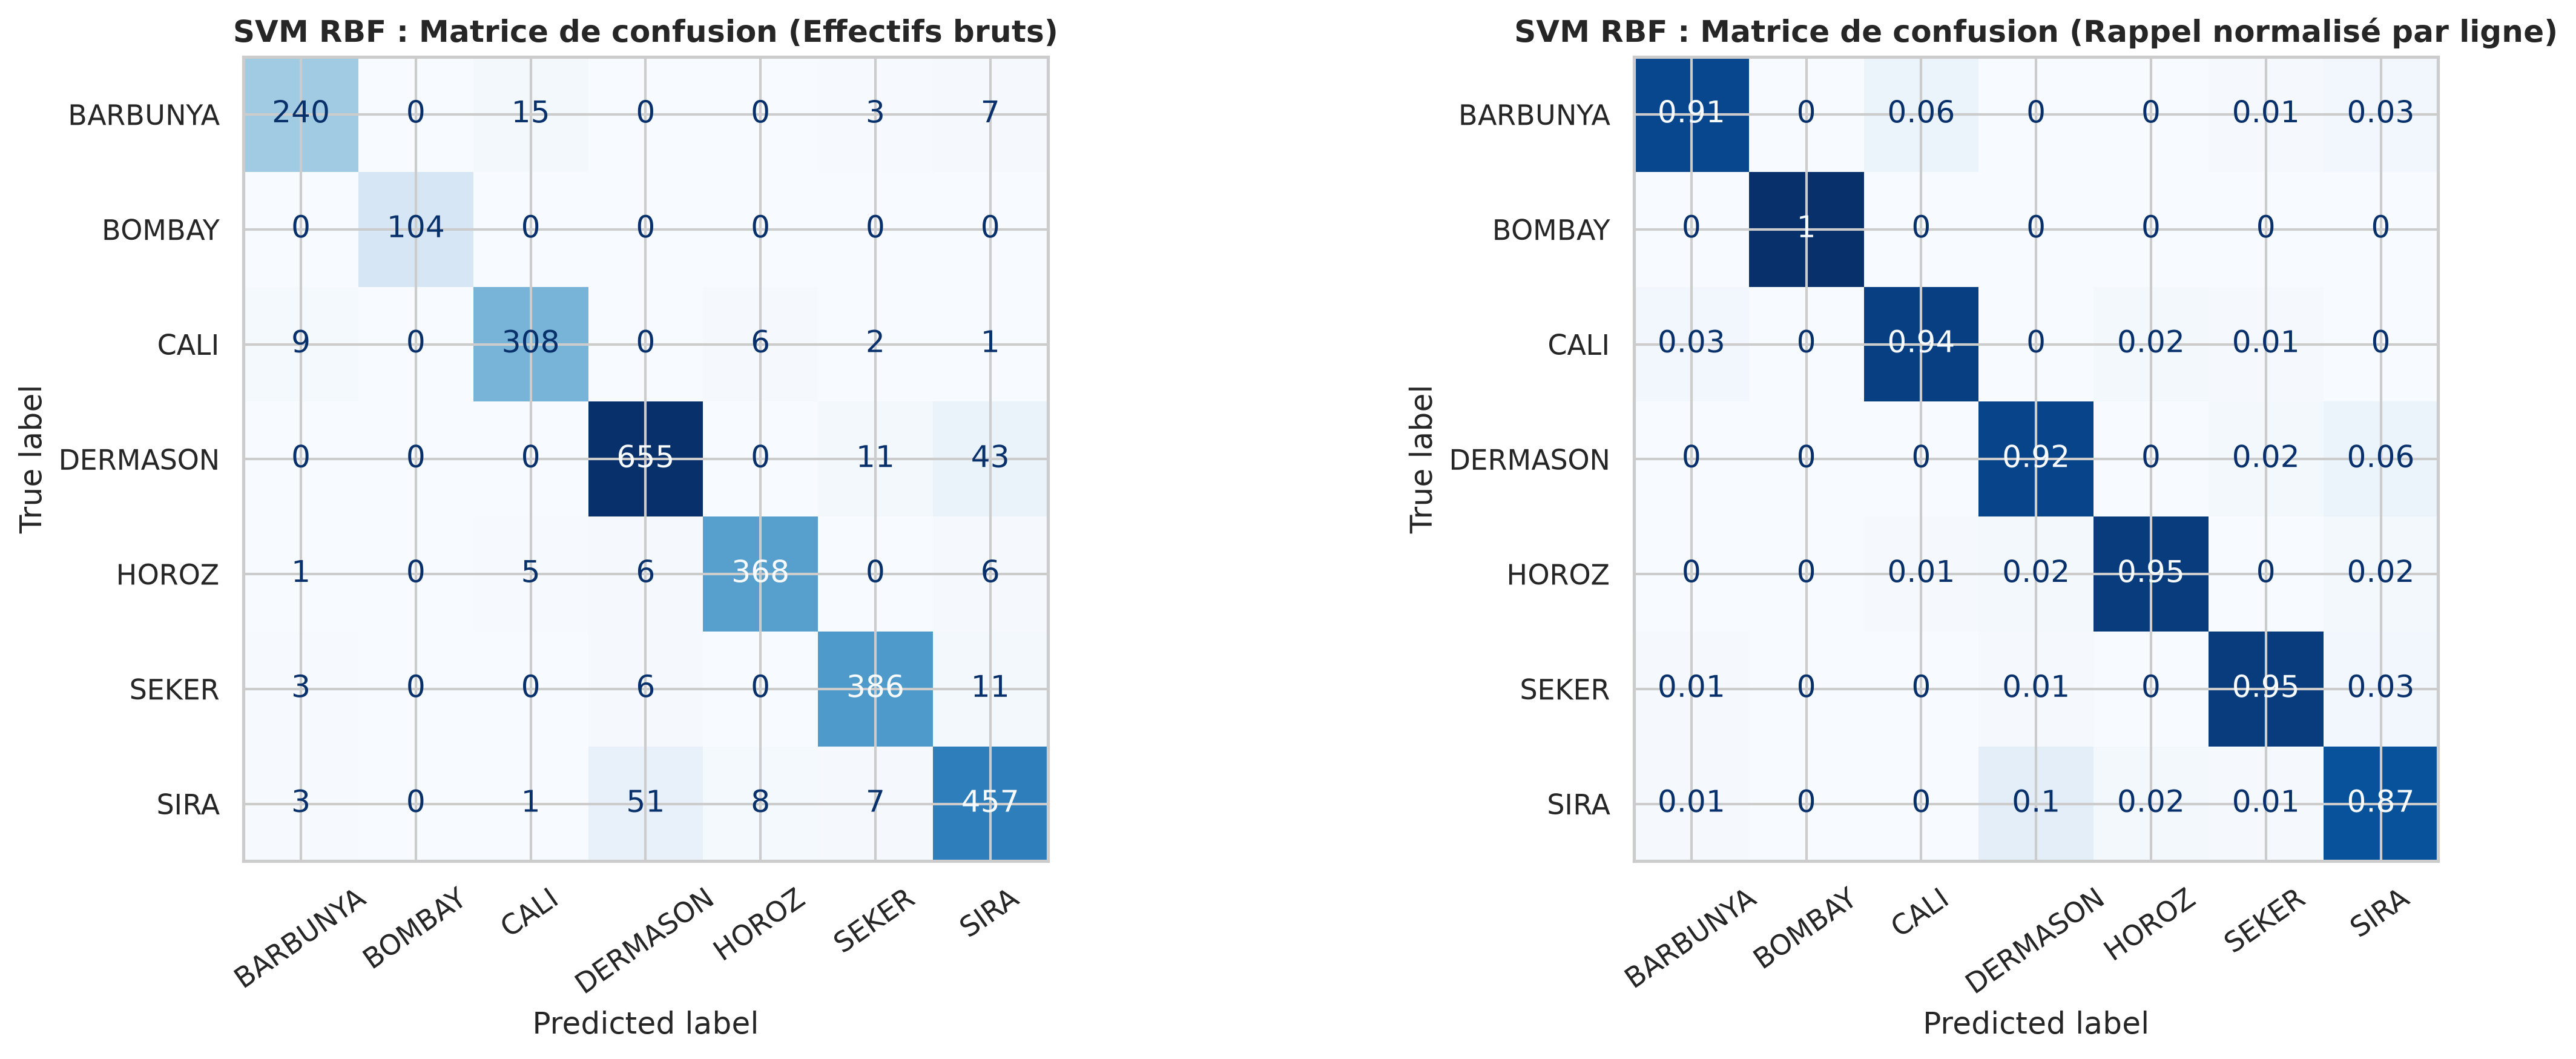
\includegraphics[width=\textwidth,height=4.6cm,keepaspectratio]{figures/07_confusion_matrix_svm_rbf.png}\\[0.1cm]
            {\scriptsize\textcolor{inseaBlue}{\textbf{Figure 4 :}} \textit{Matrice de confusion brute et normalisée (SVM RBF)}}
        \end{column}
    \end{columns}
    \note{
        \textbf{[08:30 - 09:30] Diagnostic des Confusions :}
        Voici la matrice de confusion de notre champion SVM RBF sur les 2 723 grains testés.
        Sur 205 erreurs seulement, près de la moitié (46.8%) proviennent exclusivement du couple Dermason-Sira.
        Nous avons démontré qu'il ne s'agit pas d'un défaut algorithmique mais d'une limite Bayesienne intrinsèque : dans l'espace géométrique 2D, leurs silhouettes se recouvrent physiquement.
    }
\end{frame}

% ==============================================================================
% SLIDE 11 : REPONSES AUX QUESTIONS DU PROJET ET PERSPECTIVES
% ==============================================================================
\begin{frame}{10. Synthèse des Réponses au Cahier des Charges \& Perspectives}
    \begin{columns}[T]
        \begin{column}{0.50\textwidth}
            \begin{block}{\textbf{Réponses Concluantes aux 3 Questions Clés}}
                \small
                \begin{enumerate}
                    \item \textbf{Meilleur modèle :} Le \textbf{SVM à noyau RBF} domine ($F_1 = \mathbf{0.9363}$), talonné par la Régression Logistique ($F_1 = 0.9329$) idéale pour les trieurs industriels haute cadence (2.1 ms).
                    \item \textbf{Classes les plus difficiles :} \texttt{DERMASON} ($F_1 = 0.8936$) et \texttt{SIRA} ($F_1 = 0.8778$).
                    \item \textbf{Rôle de la standardisation :} Indispensable pour SVM (+33.6 pts) et KNN (+22.2 pts), neutre sur les arbres.
                \end{enumerate}
            \end{block}
        \end{column}
        \begin{column}{0.48\textwidth}
            \begin{exampleblock}{\textbf{Bilan Méthodologique}}
                \footnotesize
                \begin{itemize}
                    \item Protocole sans fuite d'information validé.
                    \item Étalonnage rigoureux par CV 5-plis stratifiée.
                    \item 5 modèles pleinement opérationnels et documentés.
                \end{itemize}
            \end{exampleblock}
            \vspace{0.1cm}
            \begin{alertblock}{\textbf{Perspectives Scientifiques}}
                \footnotesize Intégration de descripteurs spectraux (couleur RGB / HSV, réflectance) ou de réseaux convolutifs (CNN) pour lever définitivement le verrou Dermason/Sira.
            \end{alertblock}
        \end{column}
    \end{columns}
    \note{
        \textbf{[09:30 - 10:15] Réponses \& Perspectives :}
        Pour conclure et répondre directement au cahier des charges :
        Le meilleur modèle en précision pure est le SVM RBF, mais la Régression Logistique est le champion opérationnel pour les cadences industrielles.
        Les classes les plus difficiles sont sans conteste Dermason et Sira.
        Et la standardisation est un prérequis absolu pour les modèles métriques.
        La perspective d'avenir évidente est d'exploiter la couleur et la texture via des CNN pour briser la limite Bayesienne 2D.
    }
\end{frame}

% ==============================================================================
% SLIDE 12 : REMERCIEMENTS ET QUESTIONS
% ==============================================================================
\begin{frame}[plain]
    \centering
    \vfill
    {\Huge\textbf{\textcolor{inseaBlue}{Merci pour votre attention !}}}
    \vfill
    \note{
        \textbf{[10:15 - 10:30] Fin de la Présentation :}
        Nous vous remercions chaleureusement pour votre écoute et nous sommes désormais à votre entière disposition pour répondre à vos questions et approfondir certains aspects de notre travail.
    }
\end{frame}

\end{document}